\chapter{Interpolation et approximation}\label{chap-interpolation} 


\medskip
L'\textcolorblue{interpolation} est une opération consistant à approcher une courbe qui n'est connue que par la donnée d'un nombre fini de points (ou une fonction à partir de la donnée d'un nombre fini de valeurs). 

Ainsi, l'interpolation numérique sert souvent à <<~faire émerger une courbe parmi des points~>>. Il s'agit de toutes les méthodes développées afin de mieux prendre en compte les erreurs de mesure, i.e. d'exploiter des données expérimentales pour la recherche de lois empiriques. Nous citerons par exemple la \textcolorblue{régression linéaire} et la \textcolorblue{méthode des moindres carrés} souvent bien maîtrisées. On demande à la solution du problème d'interpolation de \textcolorblue{passer par les points prescrits}, voire, suivant le type d'interpolation, de vérifier des propriétés supplémentaires (de continuité, de dérivabilité, de tangence en certains points...). Toutefois, parfois on ne demande pas à ce que l'approximation passe exactement par les points prescrits. On parle alors plutôt d'approximation. 


\begin{histoire}
Le jour du Nouvel An de 1801, l'astronome italien Giuseppe Piazzi\index[aut]{Piazzi (Giuseppe), 1746-1826, Italien} 
a découvert l'astéroïde Cérès (il a suivi sa trajectoire jusqu'au 14 février 1801). 
\sbox{\MaBoiteAvecPhotos}{\setlength{\tabcolsep}{0pt}\scriptsize%
\noindent\begin{tabular}{cccc}
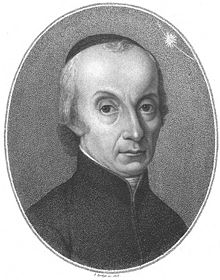
\includegraphics[height=\the\HauteurDesPhotos]{Piazzi}&
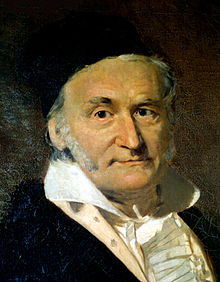
\includegraphics[height=\the\HauteurDesPhotos]{Gauss}&
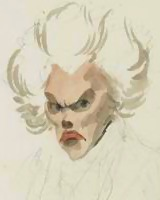
\includegraphics[height=\the\HauteurDesPhotos]{Legendre}&
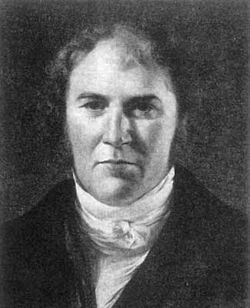
\includegraphics[height=\the\HauteurDesPhotos]{Adrain}\\
Piazzi &Gauß&Legendre &Adrain%
\end{tabular}}
\medskip
\ImageADroite{%
Durant cette année, plusieurs scientifiques ont tenté de prédire sa trajectoire sur la base des 
observations de Piazzi (à cette époque, la résolution des équations non linéaires de 
Kepler\index[aut]{Kepler (Johannes), 1571-1630, Allemand} de la cinématique est un problème 
très difficile). La plupart des prédictions furent erronées; et le seul calcul suffisamment précis pour 
permettre au baron Franz Xaver von Zach\index[aut]{Zach (Franz Xaver, Baron von -), 1754-1832, Allemand} 
(astronome allemand) de localiser à nouveau Cérès à la fin de l'année, fut celui de 
Gauß,\index[aut]{Gauß (Johann Carl Friedrich), 1777-1855, Allemand} (alors âgé 
de 24 ans). Gauß avait déjà réalisé l'élaboration des concepts fondamentaux en 1795, lorsqu'il avait
18 ans. Mais sa méthode des moindres carrés ne fut publiée qu'en 1809, lorsqu'elle parut dans le tome 2 de ses 
travaux sur la Mécanique céleste \emph{Theoria Motus Corporum Coelestium in sectionibus conicis solem ambientium}. 
Le mathématicien français Adrien-Marie Legendre\index[aut]{Legendre (Adrien-Marie), 1752-1833, Français} 
a développé indépendamment la même méthode en 1805. 
Le mathématicien américain Robert Adrain\index[aut]{Adrain (Robert), 1775-1843, Américain} 
a publié en 1808 une formulation de la méthode.}

\sbox{\MaBoiteAvecPhotos}{\setlength{\tabcolsep}{0pt}\scriptsize%
\noindent\begin{tabular}{c}
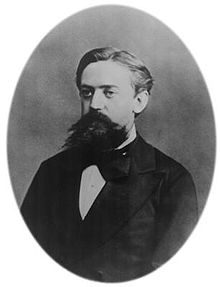
\includegraphics[height=\the\HauteurDesPhotos]{Markov}\\
Markov%
\end{tabular}}
\medskip
\ImageAGauche{En 1829, Gauß a pu donner les raisons de l'efficacité de cette méthode: 
celle-ci est optimale à l'égard de bien des critères. 
Cet argument est maintenant connu sous le nom de \textcolorblue{théorème de Gauß-Markov}\index[aut]{Markov (Andreï Andreïevitch), 1856-1922, Russe}.\\
\indent
Ce théorème dit que dans un modèle linéaire dans lequel les erreurs ont une espérance nulle, 
sont non corrélées et dont les variances sont égales, le meilleur estimateur linéaire non biaisé 
des coefficients est l'estimateur des moindres carrés. Plus généralement, le meilleur estimateur linéaire 
non biaisé d'une combinaison linéaire des coefficients est son estimateur par les moindres carrés. 
\emph{On ne suppose pas} que les erreurs possèdent une loi normale, ni qu'elles sont indépendantes 
(seulement non corrélées), ni qu'elles possèdent la même loi de probabilité.}
\end{histoire}

L'\textcolorblue{approximation} étant l'utilisation de méthodes permettant d'approcher une fonction mathématique par une suite de fonctions qui convergent dans un certain espace fonctionnel, on voit donc que ce qui a été fait dans la deuxième partie ressort bien de cela: on cherche une fonction généralement notée~$u$ qui n'est pas connue explicitement mais solution d'une équation différentielle ou d'une équation aux dérivées partielles, et l'on cherche à construire une suite de problèmes plus simples, que l'on sait résoudre à chaque étape, et telle que la suite des solutions correspondantes converge vers la solution cherchée. L'approximation peut servir aussi dans le cas où la fonction considérée est connue: on cherche alors à la remplacer par une fonction plus simple, plus régulière ou ayant de meilleures propriétés. L'intégration numérique sera détaillée un peu plus au chapitre~\ref{chap-quadrature}. Ce sont les méthodes d'approximation numériques qui sont utilisées. 

Pour en revenir à l'interpolation, la méthode des éléments finis est en elle-même une méthode d'interpolation (globale, basée sur des interpolations locales). On peut citer quelques méthodes d'interpolation telle que l'interpolation linéaire (dans laquelle deux points sucessifs sont reliés par un segment), l'interpolation cosinus (dans laquelle deux points successifs sont considérés comme les pics d'un cosinus. L'interpolation cubique ou spline (dans laquelle un polynôme de degré 3 passe par quatre points successifs: selon le type de continuité demandée plusieurs variantes existent) et de manière générale, l'interpolation polynomiale, est abordée ci-dessous. 

Faisons d'emblée une \textcolorred{mise en garde}: la plus connue des interpolations polynomiale, l'interpolation lagrangienne (approximation par les polynômes de Lagrange,\index[aut]{Lagrange (Joseph Louis, comte de -), 1736-1813, Italien} découverte initialement par Waring\index[aut]{Waring (Edward), 1736-1798, Anglais} et redécouverte par Euler)\index[aut]{Euler (Leonhard Paul), 1707-1783, Suisse} peut fort bien diverger même pour des fonctions très régulières. C'est le phénomène de Runge:\index[aut]{Runge (Carl David Tolmé), 1856-1927, Allemand} contrairement à l'intuition, \textcolorred{l'augmentation du nombre de points d'interpolation ne constitue pas nécessairement une bonne stratégie d'approximation avec certaines fonctions (même infiniment dérivables).}

\colorgris Dans le cas où l'on travaille sur le corps des complexes, une méthode d'approximation d'une fonction analytique par une fonction rationnelle est l'approximant de Padé.\index[aut]{Padé (Henri Eugène), 1863-1953, Français} Cela correspond à un développement limité qui approche la fonction par un polynôme. Tout comme les développements limités forment une suite appelée série entière, convergeant vers la fonction initiale, les approximants de Padé sont souvent vus comme une suite, s'exprimant sous la forme d'une fraction continue dont la limite est aussi la fonction initiale. En ce sens, ces approximants font partie de la vaste théorie des fractions continues. Les approximants offrent un développement dont le domaine de convergence est parfois plus large que celui d'une série entière. Ils permettent ainsi de prolonger des fonctions analytiques et d'étudier certains aspects de la question des série divergentes. En théorie analytique des nombres, l'approximant permet de mettre en évidence la nature d'un nombre ou d'une fonction arithmétique comme celle de la fonction zêta de Riemann. Dans le domaine du calcul numérique, l'approximant joue un rôle, par exemple, pour évaluer le comportement d'une solution d'un système dynamique à l'aide de la théorie des perturbations. L'approximant de Padé a été utilisé pour la première fois par Euler\index[aut]{Euler (Leonhard Paul), 1707-1783, Suisse} pour démontrer l'irrationalité de~$e$, la base du logarithme népérien. Une technique analogue a permis à Johann Heinrich Lambert\index[aut]{Lambert (Johann Heinrich), 1728-1777, Suisse} de montrer celle de~$\pi$.\colorblack



%%%%----------------------------------------------------------
\section{Quelques bases polynomiales} 
%%%%----------------------------------------------------------
%%%%----------------------------------------------------------
\subsection{Motivation} 
%%%%----------------------------------------------------------
Lorsque l'on souhaite approximer une courbe par une autre, recourir aux polynômes semble une voie naturelle. Le \textcolorblue{théorème de Taylor (1715)}\index[aut]{Taylor (Brook), 1685-1731, Anglais}\index{théorème!de Taylor} montre qu'une fonction plusieurs fois dérivable au voisinage d'un point peut être approximée par une fonction polynôme dont les coefficients dépendent uniquement des dérivées de la fonction en ce point. 
\begin{theoreme}[Développement en série de Taylor]
Soit~$I$ un intervalle de~$\RR$, $a\in I$, $E$ un espace vectoriel normé et~$f: I\rightarrow R$f une fonction dérivable en~$a$ 
jusqu’à l’ordre~$n$. Alors:
\begin{equation}
\forall x\in I, \qquad
f(x) =\sum_{k=0}^n \frac{f^{(k)}(a)}{k!}(x-a)^k + R_n(x)
\end{equation}
définit un reste~$R_n(x)$ dont le comportement s’apparente au monôme~$(x-a)^{n+1}$.
\end{theoreme}
En présentant cette formule, Taylor propose une méthode de développement en série, mais il se préoccupe peu de la 
nature du reste; il faut attendre ses successeurs pour la caractériser rigoureusement.
On désigne par \textcolorblue{théorèmes de Taylor} ou formules de Taylor plusieurs résultats et expressions pour le reste~$R_n(x)$, 
parfois renforcé par quelques hypothèses supplémentaires: 
Taylor\index[aut]{Taylor (Brook), 1685-1731, Anglais}-Young\index[aut]{Young (William Henry), 1863-1942, Anglais},
Taylor\index[aut]{Taylor (Brook), 1685-1731, Anglais}-Lagrange\index[aut]{Lagrange (Joseph Louis, comte de -), 1736-1813, Italien},
Taylor\index[aut]{Taylor (Brook), 1685-1731, Anglais}-Cauchy\index[aut]{Cauchy (Augustin Louis, baron -), 1789-1857, Français},
Taylor\index[aut]{Taylor (Brook), 1685-1731, Anglais} avec reste intégral.

Le \textcolorblue{théorème d'approximation de Weierstrass}\index[aut]{Weierstrass (Karl Theodor Wilhelm), 1815-1897, Allemand}\index{théorème!de Weierstrass} en analyse réelle dit que toute fonction continue définie sur un segment peut être approchée uniformément par des fonctions polynômes. \textcolorgris{Le théorème de Stone-Weierstrass\index[aut]{Stone (Marshall Harvey), 1903-1989, Américain}\index[aut]{Weierstrass (Karl Theodor Wilhelm), 1815-1897, Allemand}\index{théorème!de Stone-Weierstrass} généralise ce résultat aux fonctions continues définies sur un espace compact et à valeurs réelles, en remplaçant l'algèbre des polynômes par une algèbre de fonctions qui sépare les points et contient au moins une fonction constante non nulle. }

L'interpolation polynomiale consiste donc à trouver un polynôme passant par un ensemble de points donnés. Nous verrons qu'il est également possible de demander à ce que ce polynôme satisfasse à d'autres conditions.
% \footnote{% 
% \begin{tabular}{ccccc} 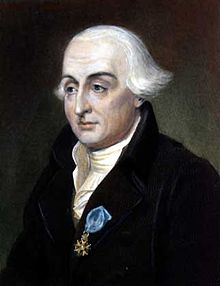
\includegraphics[height=32mm]{Lagrange}& 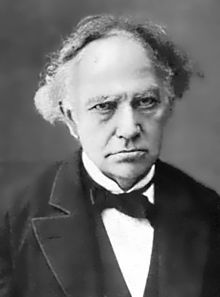
\includegraphics[height=32mm]{Hermite}& 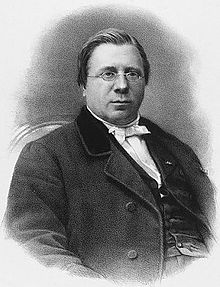
\includegraphics[height=32mm]{Bonnet}& 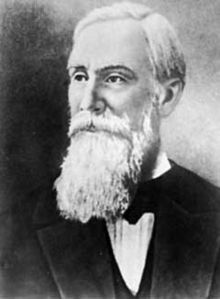
\includegraphics[height=32mm]{Tchebychev}& 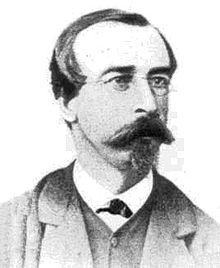
\includegraphics[height=32mm]{Laguerre}\\ Joseph Louis&%, comte de Lagrange & Charles Hermite & Pierre-Ossian Bonnet & Pafnouti Lvovitch Tchebychev & Edmond Nicolas Laguerre \\ comte de Lagrange& 1822-1901& 1819-1892& 1821-1894& 1834-1886\\ 1736-1813 \\ 
% \end{tabular}} 
 
%%%%----------------------------------------------------------
\subsection{Orthogonalité} 
%%%%----------------------------------------------------------
Une \textcolorblue{suite de polynômes orthogonaux}\index{polynôme!orthogonalité} est une suite infinie de polynômes~$P_0(x)$, $P_1(x)$, ... à coefficients réels, dans laquelle chaque~$P_n(x)$ est de degré~$n$, et telle que les polynômes de la suite sont orthogonaux deux à deux pour un produit scalaire\index{produit scalaire} de fonctions donné. Le produit scalaire\index{produit scalaire} de fonctions le plus simple est l'intégrale du produit de ces fonctions sur un intervalle borné: 
\begin{equation}
\langle f,g \rangle=\int_a^b f(x)g(x)\dd x 
\end{equation}
Plus généralement, on peut ajouter une \textcolorblue{fonction de poids}~$\varpi(x)$ dans l'intégrale. On notera bien que sur l'intervalle d'intégration~$]a,b[$, la fonction poids~$W$ doit être à valeurs finies et strictement positives, et l'intégrale du produit de la fonction poids par un polynôme doit être finie (voir espaces~$L^p$). Par contre, les bornes~$a$ et~$b$ peuvent être infinies. Il vient alors: 
\begin{equation}
 \langle f,g \rangle=\int_a^b f(x)g(x)\varpi(x)\dd x 
\end{equation}
La norme associée est définie par~$||f||=\sqrt{\langle f,f \rangle}$. Le produit scalaire\index{produit scalaire} fait de l'ensemble de toutes les fonctions de norme finie un espace de Hilbert.\index{espace!de Hilbert}\index[aut]{Hilbert (David), 1862-1943, Allemand} L'intervalle d'intégration est appelé \textcolorblue{intervalle d'orthogonalité}. 
%%%%----------------------------------------------------------
\subsection{Base naturelle} 
%%%%----------------------------------------------------------
On rappelle que~$1,X,\ldots,X^n$ est une base de~$K_n[X]$ en tant que polynômes échelonnés. 
%%%%----------------------------------------------------------
\subsection{Polynômes de Lagrange}\index[aut]{Lagrange (Joseph Louis, comte de -), 1736-1813, Italien}\index{polynôme! de Lagrange} 
%%%%----------------------------------------------------------
Connaissant~$n + 1$ points~$(x_0, y_0),\dots,(x_n, y_n)$ d'abscisses \textcolorred{distinctes}, le \textcolorblue{polynôme de Lagrange}\index[aut]{Lagrange (Joseph Louis, comte de -), 1736-1813, Italien} est l'unique polynôme de degré~$n$ passant tous les points.\index{polynôme! de Lagrange} Ce polynôme est trivialement défini par:\index{polynôme! de Lagrange} 
\begin{equation}
L(x) = \sum_{j=0}^{n} y_j \biggl(\prod_{i=0, i\neq j}^{n} \frac{x-x_i}{x_j-x_i} \biggr) 
\end{equation}
Si on note:
\begin{equation}
L(x) = \dsum_{j=0}^{n} y_j l_j(x)
\end{equation}
avec:
\begin{equation}
l_i(x) = \prod_{j=0, j\neq i}^{n} \frac{x-x_j}{x_i-x_j} = \frac{x-x_0}{x_i-x_0} \cdots \frac{x-x_{i-1}}{x_i-x_{i-1}} ~ \frac{x-x_{i+1}}{x_i-x_{i+1}} \cdots \frac{x-x_{n}}{x_i-x_{n}}
\end{equation}
alors, on remarque que: 
\begin{itemize}
\item~$l_i$ est de degré~$n$ pour tout~$i$; 
\item~$l_i(x_j) = \delta_{i,j}, 0 \leq i,j \leq n$, i.e.~$l_i(x_i) = 1$ et~$l_i(x_j) = 0$ pour~$j\ne i$ 
\end{itemize}
On en déduit immédiatement que~$\forall i$, $L(x_i) = y_i$ qui est bien la propriété recherchée par construction. 
%%%%----------------------------------------------------------
\subsection{Polynômes d'Hermite}\index[aut]{Hermite (Charles), 1822-1901, Français}\index{polynôme! d'Hermite} 
%%%%----------------------------------------------------------
Les \textcolorblue{polynômes d'Hermite}\index[aut]{Hermite (Charles), 1822-1901, Français} sont définis sous la forme dite \emph{probabiliste}:\index{polynôme! d'Hermite} 
\begin{equation}
 H_n(x)=(-1)^n \mathrm{e}^{x^2/2}\frac{\dd ^n}{\dd x^n}\mathrm{e}^{-x^2/2}
\end{equation}
ou sous la forme dite \emph{physique}: 
\begin{equation}
 \widehat{H}_n(x)=(-1)^n \mathrm{e}^{x^2}\frac{\dd^n}{\dd x^n}\mathrm{e}^{-x^2} 
\end{equation}
Les deux définitions sont liées par la propriété d'échelle suivante:
\begin{equation}
\widehat{H}_n(x) = 2^{n/2}H_n(x\sqrt{2})
\end{equation}
\colorgris
Les premiers polynômes d'Hermite\index[aut]{Hermite (Charles), 1822-1901, Français} sont les suivants:\index{polynôme! d'Hermite}
\begin{equation}
\begin{aligned}
&H_0=1\\
&H_1=x\\
&H_2=x^2-1\\
&H_3=x^3-3x\\
&H_4=x^4-6x^2+3\\
&H_5=x^5-10x^3+15x\\
&H_6=x^6-15x^4+45x^2-15
\end{aligned}
\qquad\qquad\begin{aligned}
&\widehat{H}_0=1\\
&\widehat{H}_1=2x\\
&\widehat{H}_2=4x^2-2\\
&\widehat{H}_3=8x^3-12x\\
&\widehat{H}_4=16x^4-48x^2+12\\
&\widehat{H}_5=32x^5-160x^3+120x\\
&\widehat{H}_6=64x^6-480x^4+720x^2-120
\end{aligned}
\end{equation}
\colorblack
$H_n$ est un polynôme de degré~$n$. Ces polynômes sont orthogonaux pour la mesure~$\mu$ de densité: 
\begin{equation}
 \frac{\dd \mu(x)}{\dd x} = \frac{\mathrm{e}^{-x^2/2}}{\sqrt{2\pi}}. 
\end{equation}
 Ils vérifient: 
\begin{equation}
 \int_{-\infty}^{+\infty} H_n(x)H_m(x)\,\mathrm{e}^{-x^2/2}\dd x=n!2^n\sqrt{2\pi}~\delta_{nm} 
\end{equation}
où~$\delta_{n,m}$ est le symbole de Kronecker. C'est pour ces intéressantes propriétés que cette base a été choisie en mécanique stochastique... on utilise alors la jolie expression de \textcolorblue{base de chaos polynomial}. Ces polynômes forment une base orthogonale de l'espace de Hilbert\index{espace!de Hilbert}\index[aut]{Hilbert (David), 1862-1943, Allemand}\index{produit scalaire!de~$L^2$}\index{espace!de Lebesgue}~$L^2(\CC,\mu)$ des fonctions boréliennes telles que: 
\begin{equation}
\int_{-\infty}^{+\infty}|f(x)|^2\,\frac{\mathrm{e}^{-x^2/2}}{\sqrt{2\pi}}\dd x< +\infty
\end{equation}
dans lequel le produit scalaire est donné par l'intégrale:\index{produit scalaire}\index{polynôme! orthogonalité} 
\begin{equation}
\langle f,g\rangle=\int_{-\infty}^{+\infty} f(x)\overline{g(x)}\,\frac{\mathrm{e}^{-x^2/2}}{\sqrt{2\pi}}\dd x
\end{equation}
Des propriétés analogues sont vérifiées par les polynômes de Hermite\index[aut]{Hermite (Charles), 1822-1901, Français} sous leur forme physique. 
%%%%----------------------------------------------------------
\subsection{Polynômes de Legendre}\index[aut]{Legendre (Adrien-Marie), 1752-1833, Français}\index{polynôme! de Legendre} 
%%%%----------------------------------------------------------
On appelle équation de Legendre l'équation:\index[aut]{Legendre (Adrien-Marie), 1752-1833, Français}\index{équations!de Legendre} 
\begin{equation}
\frac{\dd }{\dd x}[(1-x^{2})\frac{\dd y}{\dd x}]+n(n+1)y=0
\end{equation}
On définit le \textcolorblue{polynôme de Legendre}~$P_n$ par:\index[aut]{Legendre (Adrien-Marie), 1752-1833, Français}\index{polynôme! de Legendre} 
\begin{equation}
\frac{\dd}{\dd x}[(1-x^{2})\frac{\dd P_n(x)}{\dd x}]+n(n+1)P_n(x)=0,\quad P_n(1)=1
\end{equation}
La manière la plus simple de les définir est par la formule de récurrence de Bonnet:\index[aut]{Bonnet (Pierre-Ossian), 1819-1892, Français}~$P_0(x)=1$, $P_1(x)=x$ et:
\begin{equation}
\forall n>0, \quad (n+1)P_{n+1}(x)=(2n+1)xP_n(x) - nP_{n-1}(x)
\end{equation}
Les premiers polynômes de Legendre sont:\index[aut]{Legendre (Adrien-Marie), 1752-1833, Français}\index{polynôme! de Legendre}
\begin{equation}\colorgris
\begin{aligned}
&P_{0}(x)=1\\
&P_{1}(x)=x\\
&P_{2}(x)=\frac{1}{2}(3x^{2}-1)\\
&P_{3}(x)=\frac{1}{2}(5x^{3}-3x)\\
&P_{4}(x)=\frac{1}{8}(35x^{4}-30x^{2}+3)\\
&P_{5}(x)=\frac{1}{8}(63x^{5}-70x^{3}+15x)
\end{aligned}
\end{equation} 
Le polynôme~$P_n$ est de degré~$n$. La famille~$(P_n)_{n\leq \NN}$ est une famille de polynômes à degrés étagés, elle est donc une base de l'espace vectoriel~$\RR_n[X]$. On remarquera la propriété suivante: 
\begin{equation}
P_n(-x)=(-1)^nP_n(x)
\end{equation}
qui donne en particulier~$P_n( - 1) = ( - 1)^n$ et~$P_{2n + 1}(0) = 0$. Les polynômes orthogonaux les plus simples sont les polynômes de Legendre\index[aut]{Legendre (Adrien-Marie), 1752-1833, Français}\index{polynôme! de Legendre}\index{polynôme! orthogonalité} pour lesquels l'intervalle d'orthogonalité est~$\intff{-1}{1}$ et la fonction poids est simplement la fonction constante de valeur~$1$: ces polynômes sont orthogonaux par rapport au produit scalaire défini sur~$\RR[X]$ par:\index{produit scalaire}\index{polynôme!orthogonalité} 
\begin{equation}
\langle P,Q\rangle= \int_{-1}^{+1} P(x) Q(x)\dd x \langle P_m,P_n\rangle= \int_{-1}^{1} P_m(x)P_n(x)\dd x = 0\qquad \mathrm{pour}\qquad m \ne n 
\end{equation}
De plus, comme~$(P_n)_{n\leq N}$ est une base de~$\RR_N[X]$, on a~$P_{N+1} \in (\RR_N[X])^\bot$: 
\begin{equation}
\forall Q \in \RR_N[X],\quad \int_{-1}^{1} P_{N+1}(x)Q(x)\dd x = 0 
\end{equation}
Le carré de la norme, dans~$L^2(\intff{-1}{1})$, est:\index{produit scalaire!de~$L^2$}\index{norme!induite par un produit scalaire} 
\begin{equation}
 \|P_n\|^2=\frac{2}{2n+1}. 
\end{equation}
Ces polynômes peuvent servir à décomposer une fonction holomorphe, une fonction lipschitzienne ou à retrouver l'intégration numérique d'une fonction par la méthode de quadrature de Gauß-Legendre (voir chapitre~\ref{chap-quadrature}).\index[aut]{Legendre (Adrien-Marie), 1752-1833, Français}\index[aut]{Gauß (Johann Carl Friedrich), 1777-1855, Allemand} 
%%%%----------------------------------------------------------
\subsection{Polynômes de Tchebychev}\index[aut]{Tchebychev (Pafnouti Lvovitch), 1821-1894, Russe}\index{polynôme!de Tchebychev} 
%%%%----------------------------------------------------------
Les \textcolorblue{polynômes de Tchebychev} servent pour la convergence des interpolations de Lagrange.\index[aut]{Lagrange (Joseph Louis, comte de -), 1736-1813, Italien}\index[aut]{Tchebychev (Pafnouti Lvovitch), 1821-1894, Russe} Ils sont également utilisés dans le calcul de filtres de Tchebychev en électronique analogique.\index[aut]{Tchebychev (Pafnouti Lvovitch), 1821-1894, Russe} 

Les polynômes de Tchebychev\index[aut]{Tchebychev (Pafnouti Lvovitch), 1821-1894, Russe}\index{polynôme!de Tchebychev} constituent deux familles de polynômes (notés~$T_n$ pour la première espèce et~$U_n$ pour la seconde) définis sur l'intervalle~$\intff{-1}{1}$ par les relations trigonométriques: 
\begin{align}
&T_n(\cos(\theta))=\cos(n\theta)\\
&U_n(\cos(\theta))=\frac{\sin((n+1) \theta)}{\sin \theta} 
\end{align}
Ces deux suites sont définies par la relation de récurrence: 
\begin{equation}
\forall n\in\NN,\quad P_{n+2}(X)=2X~P_{n+1}(X)-P_n(X) 
\end{equation}
et les deux premiers termes: 
\begin{align}
&T_0=1,~T_1=X \quad \text{ pour la suite } T\\
&U_0=1,~U_1=2X \quad \text{ pour la suite } U 
\end{align}
Chacune de ces deux familles est une suite de polynômes orthogonaux\index{polynôme!orthogonalité} par rapport à un produit scalaire de fonctions assorti d'une pondération spécifique.\index{produit scalaire} 
\paragraph{Propriétés des polynômes de Tchebychev de première espèce}\index[aut]{Tchebychev (Pafnouti Lvovitch), 1821-1894, Russe}\index{polynôme! de Tchebychev} 
\begin{equation}
\forall n>0, \quad T_n(x)=\dfrac n2\dsum_{k=0}^{\left\lfloor \frac n2\right\rfloor}(-1)^k \frac{(n-k-1)!}{k!(n-2k)!}(2x)^{n-2k} 
\end{equation}
Les~$T_n$ sont orthogonaux pour le produit scalaire suivant:\index{produit scalaire}\index{polynôme!orthogonalité} 
\begin{equation}
 \int_{-1}^1 \frac{T_n(x)T_m(x)}{\sqrt{1-x^2}}\dd x= 
\begin{cases} 0&\text{ si } n\ne m\\ \pi&\text{ si } n=m=0\\ \pi/2&\text{ si } n=m\ne 0~. 
\end{cases} 
\end{equation}
\begin{equation}
\forall n, \quad T_n(1)=1,\qquad\forall n,m\in\NN,\quad \forall x\in\RR, \quad T_n(T_m(x))=T_{mn}(x) 
\end{equation}
\colorgris
Les premiers polynômes de Tchebychev de première espèce sont:\index[aut]{Tchebychev (Pafnouti Lvovitch), 1821-1894, Russe}\index{polynôme! de Tchebychev}
\begin{equation}
\begin{aligned}
&T_0 = 1 \\
&T_1 = x \\
&T_2 = 2x^2 - 1 \\
&T_3 = 4x^3 - 3x \\
& T_4 = 8x^4 - 8x^2 + 1 \\
& T_5 = 16x^5 - 20x^3 + 5x \\
& T_6 = 32x^6 - 48x^4 + 18x^2 - 1 \\
& T_7 = 64x^7 - 112x^5 + 56x^3 - 7x \\
& T_8 = 128x^8 - 256x^6 + 160x^4 - 32x^2 + 1 \\
&T_9 = 256x^9 - 576x^7 + 432x^5 - 120x^3 + 9x
\end{aligned}
\end{equation}
\colorblack
\paragraph{Propriétés des polynômes de Tchebychev de seconde espèce}\index[aut]{Tchebychev (Pafnouti Lvovitch), 1821-1894, Russe}\index{polynôme! de Tchebychev} 
\begin{equation}
\forall n\ge 0, \quad U_n(x)=\sum_{k=0}^{\left\lfloor \frac n2\right \rfloor}(-1)^k \binom{n-k}k~(2x)^{n-2k} 
\end{equation}
Les~$U_n$ sont orthogonaux\index{polynôme!orthogonalité} pour le produit scalaire\index{produit scalaire} suivant: 
\begin{equation}
\int_{-1}^1 U_n(x)U_m(x)\sqrt{1-x^2}\dd x = 
\begin{cases} 0&\text{ si } n\ne m\\ \pi/2 &\text{ si } n=m 
\end{cases} 
\quad\text{ et }\quad\forall n,\quad U_n(1)=n+1 
\end{equation}
\colorgris
Les premiers polynômes de Tchebychev de deuxième espèce sont:\index[aut]{Tchebychev (Pafnouti Lvovitch), 1821-1894, Russe}\index{polynôme! de Tchebychev}
\begin{equation}
\begin{aligned}
&U_0 = 1 \\
&U_1 = 2x \\
&U_2 = 4x^2 - 1 \\
&U_3 = 8x^3 - 4x \\
&U_4 = 16x^4 - 12x^2 + 1 \\
&U_5 = 32x^5 - 32x^3 + 6x \\
&U_6 = 64x^6 - 80x^4 + 24x^2 - 1 \\
&U_7 = 128x^7 - 192x^5 + 80x^3 - 8x \\
&U_8 = 256x^8 - 448 x^6 + 240 x^4 - 40 x^2 + 1 \\
&U_9 = 512x^9 - 1024 x^7 + 672 x^5 - 160 x^3 + 10 x
\end{aligned}
\end{equation}
\colorblack
%%%%----------------------------------------------------------
\subsection{Polynômes de Laguerre}\index[aut]{Laguerre (Edmond Nicolas), 1834-1886, Français}\index{polynôme! de Laguerre} 
%%%%----------------------------------------------------------
Les \textcolorblue{polynômes de Laguerre} apparaissent en mécanique quantique dans la partie radiale de la solution de l'équation de Schrödinger\index[aut]{Schrödinger (Erwin Rudolf Josef Alexander), 1887-1961, Autrichien} pour un atome à un électron. Ces polynômes sont les solutions de l'équation de Laguerre:\index[aut]{Laguerre (Edmond Nicolas), 1834-1886, Français}\index{polynôme! de Laguerre}\index{équations!de Laguerre} 
\begin{equation}
 xy'' + (1 - x)y' + ny = 0 
\end{equation}
qui est une équation différentielle linéaire du second ordre possédant des solutions non singulières si seulement si~$n$ est un entier positif. 

Traditionnellement notés~$L_0,L_1,\dots$ ces polynômes forment une suite de polynômes qui peut être définie par la formule de Rodrigues:\index[aut]{Rodrigues (Benjamin-Olinde), 1795-1851, Français} 
\begin{equation}
 L_n(x)=\frac{\mathrm{e}^x}{n!}\frac{\dd^n}{\dd x^n}\left(\mathrm{e}^{-x} x^n\right). 
\end{equation}
Ils sont orthogonaux\index{polynôme!orthogonalité} les uns par rapport aux autres pour le produit scalaire\index{produit scalaire}: 
\begin{equation}
\langle f,g \rangle = \int_0^\infty f(x) g(x) \mathrm{e}^{-x}\dd x 
\end{equation}
Cette propriété d'orthogonalité revient à dire que si~$X$ est une variable aléatoire distribuée exponentiellement avec la fonction densité de probabilité suivantes: 
\begin{equation}
 f(x)=\left\{
\begin{aligned}
& \mathrm{e}^{-x} && \mbox{si}\ x>0\\
&0 && \mbox{si}\ x<0
\end{aligned}\right. 
\end{equation}
alors~$E(L_n(X),L_m(X))=0$ si~$n\neq m$. 

\colorgris\noindent
Les premiers polynômes de Laguerre sont:\index[aut]{Laguerre (Edmond Nicolas), 1834-1886, Français}\index{polynôme! de Laguerre}
\begin{equation}
\begin{aligned}
&L_0 =	1\\
&L_1= 	-x+1\\
&L_2= 	\frac12 (x^2-4x+2)\\
&L_3= 	\frac16 (-x^3+9x^2-18x+6)\\
&L_4= 	\frac1{24} (x^4-16x^3+72x^2-96x+24)\\
&L_5= 	\frac1{120} (-x^5+25x^4-200x^3+600x^2-600x+120)\\
&L_6= 	\frac1{720} (x^6-36x^5+450x^4-2400x^3+5400x^2-4320x+720)
\end{aligned}
\end{equation}\colorblack
Il existe des polynômes de Laguerre\index[aut]{Laguerre (Edmond Nicolas), 1834-1886, Français} généralisés dont l'orthogonalité peut être liée à une densité de probabilité faisant intervenir la fonction Gamma. Ils apparaissent dans le traitement de l'oscillateur harmonique quantique. Ils peuvent être exprimés en fonction des polynômes d'Hermite.\index[aut]{Hermite (Charles), 1822-1901, Français}\index{polynôme! d'Hermite} 
%%%%----------------------------------------------------------
\subsection{Polynômes de Bernstein}\index[aut]{Bernstein (Sergeï{} Natanovich), 1880-1968, Russe}\index{polynôme! de Bernstein} 
%%%%----------------------------------------------------------
Les \textcolorblue{polynômes de Bernstein} permettent de donner une démonstration constructive du théorème de Stone-Weierstrass. Dans le cadre de ce cours, nous les présentons surtout car ils sont utilisés dans la formulation générale des courbes de Bézier.\index[aut]{Bézier (Pierre), 1910-1999, Français} Pour un degré~$n$, il y a~$n+1$ polynômes de Bernstein~$B^n_0, \dots, B^n_n$ définis, sur l'intervalle~$\intff{0}{1}$ par:\index{polynôme! de Bernstein} 
\begin{equation}
 B_i^n(u) = 
\begin{pmatrix} n \\ i 
\end{pmatrix} u^i \left( 1-u \right)^{n-i} \quad \text{ où les~$
\begin{pmatrix} n \\ i 
\end{pmatrix}$ sont les coefficients binomiaux.}
\end{equation}
Ces polynômes présentent quatre propriétés importantes: 
\begin{itemize}
\item Partition de l'unité:
\begin{equation}
\dsum_{i=0}^n B_i^n(u) = 1,\quad \forall u \in \intff{0}{1}
\end{equation}
\item Positivité:
\begin{equation}
B_i^n(u)\geq 0,\qquad\forall u\in \intff{0}{1},\quad\forall i\in 0,\dots,n
\end{equation}
\item Symétrie:
\begin{equation}
B_i^n(u) = B_{n-i}^n(1-u), \quad \forall u \in \intff{0}{1},\quad \forall i \in 0, \dots, n
\end{equation}
\item Formule de récurrence:
\begin{equation}
B_i^n(u) = 
\begin{cases} (1-u)B_i^{n-1}(u),& i = 0\\ (1-u)B_i^{n-1}(u) + u B_{i-1}^{n-1}(u),&\forall i \in 1, \dots, n-1\\ uB_{i-1}^{n-1}(u),& i = n 
\end{cases},\quad \forall u \in \intff{0}{1}
\end{equation}
\end{itemize}
On notera la grande ressemblance de ces polynômes avec la loi binomiale. 
%%%%----------------------------------------------------------
\section{Interpolation polynomiale} 
%%%%---------------------------------------------------------- 
%%%%----------------------------------------------------------
\subsection{Interpolation de Lagrange} 
%%%%----------------------------------------------------------
Dans la version la plus simple (\textcolorblue{interpolation lagrangienne}), on impose simplement que le polynôme passe par tous les points donnés. On obtient les polynômes de Lagrange tels que présentés juste avant. \index[aut]{Lagrange (Joseph Louis, comte de -), 1736-1813, Italien}\index{polynôme!de Lagrange} Le théorème de l'unisolvance (voir paragraphe~\ref{Sec-unisolvance}) précise qu'il n'existe qu'un seul polynôme de degré~$n$ au plus défini par un ensemble de~$n+1$ points. 

L'\textcolorblue{erreur d'interpolation} lors de l'approximation d'une fonction~$f$ (donnée par les points~$(x_i,y_i=f(x_i))$) par un polynôme de Lagrange~$p_n$ est donnée par une formule de type Taylor-Young:\index[aut]{Taylor (Brook), 1685-1731, Anglais}\index[aut]{Young (William Henry), 1863-1942, Anglais} Si~$f$ est~$n+1$ fois continûment différentiable sur~$I=[\min(x_0,\ldots,x_n,x),\max(x_0,\ldots,x_n,x)]$, alors:
\begin{equation}
f(x) - p_n(x) = \frac{f^{(n+1)}(\xi)}{(n+1)!} \prod_{i=0}^n (x-x_i) \quad \text{ avec }\quad \xi \in I
\end{equation}
Dans le cas particulier où~$x_i = x_0 + ih$ (points uniformément répartis), il se produit en général une \textcolorred{aggravation catastrophique de l'erreur d'interpolation}, connue sous le nom de \textcolorblue{phénomène de Runge}\index[aut]{Runge (Carl David Tolmé), 1856-1927, Allemand} lorsqu'on augmente le nombre de points pour un intervalle~$[x_0,x_n]$, donné (on a alors~$\xi\in]-1,1[$). 

\textcolorblue{Pour limiter le phénomène de Runge},\index[aut]{Runge (Carl David Tolmé), 1856-1927, Allemand} i.e. pour minimiser l'oscillation des polynômes interpolateurs, on peut utiliser les abscisses de Tchebychev\index[aut]{Tchebychev (Pafnouti Lvovitch), 1821-1894, Russe} au lieu de points équirépartis pour interpoler. Dans ce cas, on peut montrer que l'erreur d'interpolation décroît lorsque~$n$ augmente. On peut aussi préférer utiliser des splines ppour approximer la fonction~$f$ (ce sont des polynômes par morceaux définis plus bas). Dans ce cas, pour améliorer l'approximation, on augmente le nombre de morceaux et non le degré des polynômes. 
 
%%%%----------------------------------------------------------
\subsection{Interpolation par Spline} 
%%%%----------------------------------------------------------
Une \textcolorblue{spline} est une fonction définie par morceaux par des polynômes. Comme mentionné au dessus, la méthode des splines est souvent préférée à l'interpolation polynomiale, car on obtient des résultats similaires en se servant de polynômes ayant des degrés inférieurs, tout en évitant le phénomène de Runge. De plus, leur simplicité d'implémentation les rend très populaires et elles sont fréquemment utilisées dans les logiciels de dessin. 

Une courbe spline est une fonction polynomiale par morceaux définie sur un intervalle~$\intff{a}{b}$ divisé en sous intervalles~$\intff{t_{i-1}}{t_i}$ tels que~$a = t_0 < t_1 < \ldots < t_{k-1} < t_k = b$. On la note~$S: \intff{a}{b}\to \RR$. Sur chaque intervalle~$\intff{t_{i-1}}{t_i}$ on définit un polynôme~$ P_i: \intff{t_{i-1}}{t_i} \to \RR$. Cela entraine pour une spline à~$k$ intervalles:~$S(t) = P_1 (t)$, $t_0 \le t < t_1$, $S(t) = P_2 (t)$, $t_1 \le t < t_2,\ldots,S(t) = P_k (t)$, $t_{k-1} \le t \le t_k$. 

Le \textcolorblue{degré de la spline} est défini comme étant celui du polynôme~$P_i (t)$ de plus haut degré. Si tous les polynômes ont le même degré, on dit que la spline est uniforme. Dans le cas contraire, elle est non uniforme. 

Tout polynôme étant~$C^\infty$, la \textcolorblue{continuité d'une spline} dépend de la continuité au niveau de la jointure des courbes polynômes. Si~$\forall i$ tel que~$1 \le i \le k$ et~$\forall j$ tel que~$0 \le j \le n$ l'égalité suivante est vérifiée: 
\begin{equation}
 P_i^{(j)} (t_i) = P_{i+1}^{(j)} (t_i)
\end{equation}
alors la spline est~$C^n$. 
 
%%%%----------------------------------------------------------
\subsection{Interpolation d'Hermite}
%%%%----------------------------------------------------------
L'\textcolorblue{interpolation d'Hermite}\index[aut]{Hermite (Charles), 1822-1901, Français} consiste à chercher un polynôme\index{polynôme! d'Hermite} qui non seulement prend les valeurs fixées en les abscisses données, mais dont également la dérivée, donc la pente de la courbe, prend une valeur imposée en chacun de ces points. Naturellement, il faut pour cela un polynôme de degré supérieur au polynôme de Lagrange. \index[aut]{Lagrange (Joseph Louis, comte de -), 1736-1813, Italien}\index{polynôme! de Lagrange} On peut aussi imposer encore la valeur des dérivées secondes, troisièmes, etc. en chaque point. La démarche de l'interpolation newtonienne\index[aut]{Newton (Isaac, Sir -), 1643-1727, Anglais} utilisant les différences divisées est particulièrement adaptée pour construire ces polynômes. 
 
%%%%----------------------------------------------------------
\section{Méthodes d'approximation}
%%%%---------------------------------------------------------- 
%%%%----------------------------------------------------------
\subsection{Courbe de Bézier}\index[aut]{Bézier (Pierre), 1910-1999, Français}
%%%%----------------------------------------------------------
\begin{histoire}Pierre Bézier (ingénieur de l'École nationale supérieure d'arts et métiers en 1930 et de l'École supérieure d'électricité en 1931, il reçoit le titre de docteur en mathématiques de l'université de Paris en 1977) est connu pour son invention des courbes et surfaces de Bézier, couramment utilisées en informatique. 

\sbox{\MaBoiteAvecPhotos}{\setlength{\tabcolsep}{0pt}\scriptsize%
\begin{tabular}{c}%
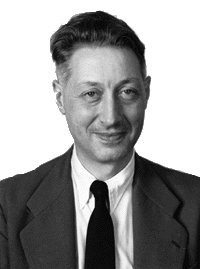
\includegraphics[height=\the\HauteurDesPhotos]{Bezier}\\%
Bézier%
\end{tabular}}
\medskip
\ImageADroite{%
Entré chez Renault en 1933, il y fera toute sa carrière jusqu'en 1975 au poste de directeur des méthodes mécaniques. Il y conçoit, en 1945, des machines transferts pour la ligne de fabrication des Renault 4CV, et, en 1958, l'une des premières machines à commande numérique d'Europe, une fraiseuse servant aux maquettes. Sa préoccupation était de créer un moyen simple et puissant pour modéliser des formes et faciliter la programmation des machines à commande numérique. Le problème auquel il s'attaque est celui de la modélisation des surfaces en trois dimensions, les commandes numériques se contentant jusqu'alors de courbes en deux dimensions. La solution qu'il cherche est celle d'une interface intuitive accessible à tout utilisateur. Il décide de considérer classiquement les surfaces comme une transformation de courbes. Son exigence de s'adapter au dessinateur et non de contraindre le dessinateur à devenir calculateur, l'amène à une inversion géniale, déduire le calcul à partir du dessin et non le dessin à partir du calcul. Il invente alors la poignée de contrôle, curseur de déplacement des courbes d'un dessin informatisé transmettant automatiquement les variations de coordonnées au processeur. Ces poignées de contrôle sont toujours utilisées aujourd'hui.}

Les courbes de Bézier sont des courbes polynomiales paramétriques. \index[aut]{Bézier (Pierre), 1910-1999, Français} Elles ont de nombreuses applications dans la synthèse d'images et le rendu de polices de caractères (Pierre Bézier a travaillé sur les deux sujets). Ses recherches aboutirent à un logiciel, Unisurf, breveté en 1966. Il est à la base de tous les logiciels créés par la suite. Les concepts de CAO et de CFAO venaient de prendre forme. Ultérieurement, l'un des développeurs d'Apple, John Warnock,\index[aut]{Warnock (John Edward), 1940- , Américain} réutilise les travaux de Pierre Bézier pour élaborer un nouveau langage de dessin de polices: Postscript. Il crée ensuite en 1982, avec Charles M. Geschke,\index[aut]{Geschke (Charles M.), 1939-, Américain} la société Adobe pour lancer un logiciel de dessin dérivé de ces résultats: Illustrator. 
\end{histoire}

Notons que les splines existaient avant Bézier\index[aut]{Bézier (Pierre), 1910-1999, Français}, mais leur défaut était de changer d'aspect lors d'une rotation de repère, ce qui les rendait inutilisables en CAO. Bézier partit d'une approche géométrique fondée sur la linéarité de l'espace euclidien et la théorie, déjà existante, du barycentre: si la définition est purement géométrique, aucun repère n'intervient puisque la construction en est indépendante. Les splines conformes aux principes de Bézier seront par la suite nommées B-splines.  

Pour~$n+1$ \textcolorblue{points de contrôle}~$(P_0, \dots, P_n)$ on définit une \textcolorblue{courbe de Bézier} par l'ensemble des points:
\begin{equation}
b(t)=\dsum_{i=0}^n B_i^n(t)\cdot P_i\quad\text{ avec }\quad t \in\intff{0}{1}
\end{equation}
où les~$B_i^n$ sont les polynômes de Bernstein. La suite des points~$P_0, \ldots, P_n$ forme le \textcolorblue{polygone de contrôle de Bézier}. 

Chaque point de la courbe peut être vu alors comme un barycentre des~$n+1$ points de contrôle pondérés d'un poids égal au polynôme de Bernstein.\index[aut]{Bernstein (Sergeï Natanovich), 1880-1968, Russe}\index{polynôme!de Bernstein} 
Les principales propriétés des courbes de Bézier sont les suivantes:
\begin{itemize}
\item la courbe est à l'intérieur de l'enveloppe convexe des points de contrôle;\index[aut]{Bézier (Pierre), 1910-1999, Français} 
\item la courbe commence par le point~$P_0$ et se termine par le point~$P_n$, mais ne passe pas \emph{a priori} par les autres points de contrôle;
\item~$\vect{P_0P_1}$ est le vecteur tangent à la courbe en~$P_0$ et~$\vect{P_{n-1}P_n}$ au point~$P_n$;
\item une courbe de Bézier est~$C^{\infty}$;
\item la courbe de Bézier est un segment si et seulement si les points de contrôle sont alignés;
\item chaque restriction d'une courbe de Bézier est aussi une courbe de Bézier;
\item un arc de cercle (ni même aucun arc de courbe conique, en dehors du segment de droite) ne peut pas être décrit par une courbe de Bézier, quel que soit son degré;
\item \textcolorred{le contrôle de la courbe est global: modifier un point de contrôle modifie toute la courbe, et non pas un voisinage du point de contrôle;}
\item pour effectuer une transformation affine de la courbe, il suffit d'effectuer la transformation sur tous les points de contrôle. 
\end{itemize}
%%%%----------------------------------------------------------
\subsection{B-Spline}
%%%%----------------------------------------------------------
Une \textcolorblue{B-spline} est une combinaison linéaire de splines positives à support compact minimal. Les B-splines sont la généralisation des courbes de Bézier, elles peuvent être à leur tour généralisées par les NURBS.\index[aut]{Bézier (Pierre), 1910-1999, Français} Étant donné~$m+1$ points~$t_i$ dans~$\intff{0}{1}$ tels que~$0\le t_0\le t_1\le\ldots\le t_m\le 1$, une courbe spline de degré~$n$ est une courbe paramétrique~$S:\intff{0}{1}\to\mathbb{R}^d$, composée de fonctions \textcolorblue{B-splines} de degré~$n$: 
\begin{equation}
S(t)=\sum_{i=0}^{m-n-1}b_{i,n}(t)\cdot P_{i},\quad t \in \intff{0}{1}
\end{equation}
où les~$P_i$ forment un polygone appelé \textcolorblue{polygone de contrôle}. Le nombre de points composant ce polygone est égal à~$m-n$. Les~$m-n$ fonctions B-splines de degré~$n$ sont définies par récurrence sur le degré inférieur: 
\begin{align}
&b_{j, 0}(t)= \left\{ 
\begin{aligned} &1 && \text{ si } \quad t_j \leqslant t < t_{j + 1} \\
&0 && \text{ sinon } 
\end{aligned} \right.\\
&b_{j, n}(t)= \frac{t - t_j}{t_{j + n} - t_j} b_{j, n - 1}(t) + \frac{t_{j + n + 1} - t}{t_{j + n + 1} - t_{j + 1}} b_{j + 1, n - 1}(t)
\end{align}
Quand les points sont équidistants, les B-splines sont dites uniformes. C'est le cas des courbes de Bézier qui sont des B-splines uniformes, dont les points~$t_i$ (pour~$i$ entre~$0$ et~$m$) forment une suite arithmétique de~$0$ à~$1$ avec un pas constant~$h=1/m$, et où le degré~$n$ de la courbe de Bézier ne peut être supérieur à~$m$). 

\textcolorgris{Par extension, lorsque deux points successifs~$t_j$ et~$t_{j+1}$ sont confondus, on pose~$0/0 = 0$: cela a pour effet de définir une discontinuité de la tangente, pour le point de la courbe paramétré par une valeur de~$t$, donc d'y créer un sommet d'angle non plat.} \textcolorgreen{Toutefois il est souvent plus simple de définir ce B-spline étendu comme l'union de deux B-splines définis avec des points distincts, ces splines étant simplement joints par ce sommet commun, sans introduire de difficulté dans l'évaluation paramétrique ci-dessus des B-splines pour certaines valeurs du paramètre~$t$. Mais cela permet de considérer alors tout polygone simple comme un B-spline étendu.}
 
La forme des fonctions de base est déterminée par la position des points. La courbe est à l'intérieur de l'enveloppe convexe des points de contrôle. Une B-spline de degré~$n$, $b_{i,n}(t)$ est non nulle dans l'intervalle~$\intff{t_i}{t_{i+n+1}}$: 
\begin{equation}
b_{i,n}(t) =\left\{\begin{aligned}
&>0 && \text{ si } \quad t_{i} \leqslant t < t_{i+n+1} \\
&0 && \text{ sinon } 
\end{aligned}\right. 
\end{equation}
En d'autres termes, \textcolorblue{déplacer un point de contrôle ne modifie que localement l'allure de la courbe}. Par contre, les B-splines ne permettent pas de décrire un arc de courbe conique. 
%%%%----------------------------------------------------------
\subsection{B-splines rationnelles non uniformes} 
%%%%----------------------------------------------------------
Ces objets couramment nommés \textcolorblue{NURBS}, pour Non-Uniform Rational Basis Splines, correspondent à une généralisation des B-splines car ces fonctions sont définies avec des points en coordonnées homogènes. Les coordonnées homogènes, introduites par Möbius,\index[aut]{Möbius (August (us) Ferdinand), 1790-1868, Allemand} rendent les calculs possibles dans l'espace projectif comme les coordonnées cartésiennes le font dans l'espace euclidien. Ces coordonnées homogènes sont largement utilisées en infographie ou en CAO car elles permettent la représentation de scènes en trois dimensions. Les NURBS parviennent à ajuster des courbes qui ne peuvent pas être représentées par des B-splines uniformes. Ils permettent même une représentation exacte de la totalité des arcs coniques ainsi que la totalité des courbes et surfaces polynomiales, avec uniquement des paramètres entiers ou rationnels si les NURBS passent par un nombre limité mais suffisant de points définis dans un maillage discret de l'espace. 

Les fonctions NURBS de degré~$d$ sont définies par la formule doublement récursive de Cox-de Boor (formulation trouvée de manière indépendante par M.G. Cox en 1971 et C. de Boor en 1972):\index[aut]{Cox (M. G.)}\index[aut]{de Boor (Carl-Wilhelm Reinhold), 1937-, Américain} 
\begin{equation}
\left\{\begin{aligned}
&b_{j,0}(t)=
\left\{\begin{aligned}
& 1 && \text{ si }\quad t_j \leq t < t_{j+1} \\
& 0 && \text{ sinon } 
\end{aligned}\right.\\ 
&b_{j,d}(t)= \dfrac{t-t_j}{t_{j+d}-t_j} b_{j,d-1}(t)+\dfrac{t_{j+d+1}-t}{t_{j+d+1}-t_{j+1}}b_{j+1,d-1}(t)
\end{aligned}\right. 
\end{equation}
où les~$t_j$ sont des points. Lorsque plusieurs points~$t_j$ sont confondus, on peut encore poser~$0/0=0$ comme pour les B-splines. 